\subsubsection{UC16 - Visione ad alto livello - utente sviluppatore}
\begin{figure}[h]
	\centering
	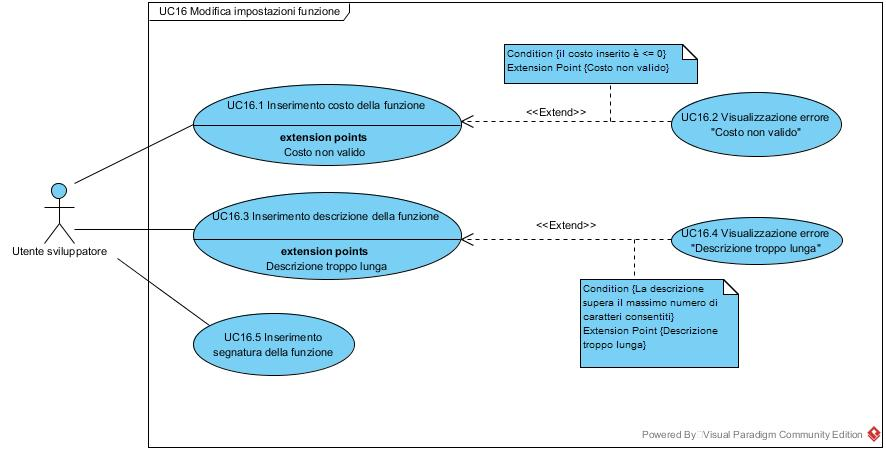
\includegraphics[width=\linewidth]{res/img/UC16.jpg}
	\caption{Diagramma UC16 - visione ad alto livello - utente sviluppatore}
\end{figure}
\begin{itemize}
	\item \textbf{Attori primari:} Utente sviluppatore;
	\item \textbf{Descrizione:} l'utente che ha eseguito l'autenticazione a \textit{Etherless} mediante l'utenza \textit{Ethereum\glo} e, disponendo di una funzione JavaScript da rendere utilizzabile sulla piattaforma, ha accesso ai comandi dedicati agli utenti sviluppatori;
	\item \textbf{Pre-condizioni:} l'utente ha eseguito l'accesso al sistema e e possiede una funzione JavaScript da caricare sulla piattaforma;
	\item \textbf{Post-condizioni:} l'utente potrà eseguire i comandi messi a disposizione per gli utenti sviluppatori;
	\item \textbf{Scenario principale:}
	\begin{enumerate}
		\item L'utente può eseguire il deploy di una propria funzione JavaScript (UC17);
		\item L'utente può modificare le impostazione di una sua funzione presente nel sistema (UC18);
		\item L'utente può rimuovere una sua funzione presente nel sistema (UC19);
		\item L'utente può aggiornare il codice di una sua funzione presente nel sistema (UC20);
		\item L'utente può eseguire le operazioni descritte da UC18, UC19, UC20 solo se la funzione esiste all'interno della piattaforma, quindi quando non si presenta UC21.
	\end{enumerate}
\end{itemize}
